\documentclass[10pt,landscape,a4paper]{article}
\usepackage[utf8]{inputenc}
% \usepackage[ngerman]{babel}
\usepackage[T1]{fontenc}
%\usepackage[LY1,T1]{fontenc}
%\usepackage{frutigernext}
%\usepackage[lf,minionint]{MinionPro}
\usepackage{tikz}
\usetikzlibrary{shapes,positioning,arrows,fit,calc,graphs,graphs.standard}
\usepackage[nosf]{kpfonts}
\usepackage[t1]{sourcesanspro}
\usepackage{multicol}
\usepackage{wrapfig}
\usepackage[top=3mm,bottom=3mm,left=3mm,right=3mm]{geometry}
\usepackage[framemethod=tikz]{mdframed}
\usepackage{microtype}
\usepackage{pdfpages}
\usepackage{algpseudocodex}
% \usepackage{algorithmic, algorithm} % Pseudocode
\usepackage{quiver}
\usepackage{dsfont} % extra signs

\let\bar\overline

\begin{document}
\include{inhalt/def.tex}
\footnotesize
\small
\begin{multicols*}{4}
\header
\section{Intro \& Bandits}

Let\textquotesingle s say you have 4 different options. For each choice
there is a reward, and there is also a long-term reward. At each time
step \(t\) the agent chooses an action \(A_t\) and receives some reward
\(R_t\)

\begin{itemize}
\item
  There are \(k\) available options
\item
  The expected reward of some action a is as follows (this is often
  defined as "action value"):
\end{itemize}

\begin{equation}
Q_t(a) = \frac{\text{Sum of R when $a$ chosen before $t$}}{\text{\# times $a$ chosen before $t$}}
\tag{Expected reward of a}
\end{equation}

Given the estimated value of all possible actions, we take the action
with the largest \(Q_t(a)\) (greedy)

\begin{equation}
\label{eq:3}
A_t = argmax_a(Q_t(a))
\end{equation}

\subsection{Saving rewards}\label{saving-rewards}

You do not need to save all historical rewards of an action, to estimate
\(Q_t\) We just upadte \(Q_{t-1}\) to \(Q_t\) when a new reward
\(R_{t-1}\) comes in:

\begin{equation}
\label{eq:4}
Q_t = Q_{t-1} + \frac{1}{t-1} ( R_{t-1} - Q_{t-1})
\end{equation}

This is cheap in terms of memory and computation. A general form we will
see often:

\begin{equation}
\label{eq:5}
\text{NewEstimate} = \text{ OldEstimate + stepSize(Target - Oldestimate)}
\end{equation}

\subsection{Greedy vs other
approaches}\label{greedy-vs-other-approaches}

The reward distribution may not be linear. You need to look at
exploration vs exploitation of the reward structure. This is an
important tradeoff in RL, at each point you can either:

\begin{enumerate}
\item
  Exploit the information you have: pick the action believed to be best
\item
  Explore: try out another action, maybe get new information
\end{enumerate}

By taking a greedy approach, we are only diong exploitation. A
straightforward way to add some exploration, is called the
\(\epsilon - greedy\) action selection:

\begin{itemize}
\item
  Most of the time we are greedy
\item
  For each action, with some small probability \(\epsilon\) we select an
  action uniformely at random
\item
  As \(t\) goes to infinity, so does the number of times each action is
  tried. So our estimates \(Q_t(a)\) will converge slowly to
  \(q_{*}(a)\).

\end{itemize}

\subsection{A k-armed bandit algorithm}

\begin{mdframed}
  
\textbf{$\varepsilon$-greedy k-armed bandit algorithm}
\begin{algorithmic}
\State Initialize $Q(a) \leftarrow 0$ and $N(a) \leftarrow 0$ for all actions $a = 1, \ldots, k$
\For{each step $t = 1, 2, \ldots, T$}
    \State With probability $\varepsilon$ select a random action $A_t$
    \State Otherwise select $A_t = \arg\max_a Q(a)$
    \State Take action $A_t$ and observe reward $R_t$
    \State Update:
    \State \hspace{1em} $N(A_t) \leftarrow N(A_t) + 1$
    \State \hspace{1em} $Q(A_t) \leftarrow Q(A_t) + \frac{1}{N(A_t)} (R_t - Q(A_t))$
\EndFor
\end{algorithmic}
\end{mdframed}

\subsection{How does \(\epsilon\) affect learning?}

The parameter \(\epsilon\) is related to the exploration strategy of the
multi-armed bandits algorithm. A smalll \(\epsilon\) (less exploration)
can lead to eventual better performance.

\begin{itemize}
\item
  \(\epsilon\) too small: Needs a long time to find optimal solution,
  likely to get stuck in suboptimal action
\item
  \(\epsilon\) too large: in the long run, keeps making wrong moves even
  if it has already found the most optimal action.
\end{itemize}

\section{Markov Decision Process}

\section{Dynamic Programming}
\begin{mdframed}
\textbf{Iterative Policy Evaluation Algorithm}
\begin{algorithmic}
\State Input: policy $\pi$ to be evaluated
\State Initialize $V(s) = 0$ for all $s \in \mathcal{S}^+$ (arbitrarily, except $V(terminal) = 0$)
\Repeat
  \State $\Delta \leftarrow 0$
  \For{each $s \in \mathcal{S}$}
    \State $v \leftarrow V(s)$
    \State $V(s) \leftarrow \sum_a \pi(a|s) \sum_{s',r} p(s',r|s,a)[r + \gamma V(s')]$
    \State $\Delta \leftarrow \max(\Delta, |v - V(s)|)$
  \EndFor
\Until{$\Delta < \theta$ (a small threshold determining accuracy)}
\State Output: $V \approx v_\pi$
\end{algorithmic}
\end{mdframed}
\section{Monte Carlo}
\begin{mdframed}
  
\textbf{First-visit MC prediction Algorithm}
\begin{algorithmic}
\State Input: policy $\pi$ to be evaluated
\State Initialize:
\State \hspace{1em} $V(s) \in \mathbb{R}$ arbitrarily for all $s \in \mathcal{S}$
\State \hspace{1em} $Returns(s) \leftarrow$ empty list for all $s \in \mathcal{S}$
\Repeat
  \State Generate an episode following $\pi$: $S_0, A_0, R_1, S_1, A_1, R_2, \ldots, S_{T-1}, A_{T-1}, R_T$
  \State $G \leftarrow 0$
  \For{each step $t = T-1, T-2, \ldots, 0$}
    \State $G \leftarrow \gamma G + R_{t+1}$
    \If{\textcolor{blue}{$S_t$ does not appear in $S_0, S_1, \ldots, S_{t-1}$}
    \footnote{Note that without this line, this algo becomes full MC prediction}}
      \State Append $G$ to $Returns(S_t)$
      \State $V(S_t) \leftarrow$ average$(Returns(S_t))$
    \EndIf
  \EndFor
\Until{forever}
\end{algorithmic}
\end{mdframed}

This algorithm tries to estimate $v_{\pi}(s)$, the value of some state $s$ under policy $\pi$,
given a set of episodes obtained by following policy $\pi$ and passing through $s$.
Note that $s$ may be visited multiple times in the same episode.
We call each visit of some episode $s$ a 'visit' of that state, and first-visit 
just evaluates following first visits to $s$ in the episode, averaging them.
Every-visit MC prediction is just the same algorithm, without the check for $S_t$ having occurred earlier in the episode.

\subsection{Monte Carlo Control}
Monte Carlo Control keeps track of an alternate approximate value function, 
and that value function is then altered every iteration to more closely approximate the real value function.

Policy improvement of this control algorithm is done by making the policy greedy
with respect to the current value function.

For any action-value function $q$, the corresponding greedy policy is the one that, 
foreach $s \in S$, chooses the action with maximal value:
\begin{equation}
  \pi(s) \doteq arg max_a q(s,a)
\end{equation}

Policy improvement can then be done by constructing each $\pi_{k+1}$ as
the greedy policy, with respect to $q_{pi_{k}}$

\begin{mdframed}
  
\textbf{Monte Carlo ES (Exploring Starts) Algorithm}
\begin{algorithmic}
\State Initialize:
\State \hspace{1em} $Q(s,a) \in \mathbb{R}$ arbitrarily for all $s \in \mathcal{S}, a \in \mathcal{A}(s)$
\State \hspace{1em} $\pi(s) \leftarrow$ arbitrary policy for all $s \in \mathcal{S}$
\State \hspace{1em} $Returns(s,a) \leftarrow$ empty list for all $s \in \mathcal{S}, a \in \mathcal{A}(s)$
\Repeat
  \State Choose $S_0 \in \mathcal{S}$ and $A_0 \in \mathcal{A}(S_0)$ randomly such that all pairs have probability $> 0$
  \State Generate an episode from $S_0, A_0$ following $\pi$: $S_0, A_0, R_1, S_1, A_1, R_2, \ldots, S_{T-1}, A_{T-1}, R_T$
  \State $G \leftarrow 0$
  \For{each step $t = T-1, T-2, \ldots, 0$}
    \State $G \leftarrow \gamma G + R_{t+1}$
    \If{$(S_t, A_t)$ does not appear in $(S_0, A_0), (S_1, A_1), \ldots, (S_{t-1}, A_{t-1})$}
      \State Append $G$ to $Returns(S_t, A_t)$
      \State $Q(S_t, A_t) \leftarrow$ average$(Returns(S_t, A_t))$
      \State $\pi(S_t) \leftarrow \arg\max_a Q(S_t, a)$
    \EndIf
  \EndFor
\Until{forever}
\end{algorithmic}
\end{mdframed}
\section{TD Learning}

TD Learning is a combination of ideas from Monte Carlo and Dynamic Programming.
We update estimates based in part on other learned estimates, without waiting for a final outcome.

Monte Carlo methods need to wait until the end of the episode until determining $V(S_t)$ increment,
because only then do we know what $G_t$ is going to be.
But! TD methods wait only until the next time step, at $t + 1$ they immediately form a target and make a useful update using $R_{t+1}$
\begin{equation}
  V(S_t) \leftarrow V(S_t) + \alpha [ R_{t+1} + \gamma V(S_{t+1}) - V(S_t)]
\end{equation}

Note that this is a special case of the TD($\gamma$) algorithm:\\
\begin{mdframed}
  
\textbf{Tabular TD(0) for estimating $v_\pi$}
\begin{algorithmic}
\State Input: the policy $\pi$ to be evaluated
\State Algorithm parameter: step size $\alpha \in (0,1]$
\State Initialize $V(s)$, for all $s \in \mathcal{S}^+$, arbitrarily except that $V(terminal) = 0$
\Repeat
  \State Initialize $S$
  \Repeat
    \State $A \leftarrow$ action given by $\pi$ for $S$
    \State Take action $A$, observe $R$, $S'$
    \State $V(S) \leftarrow V(S) + \alpha [R + \gamma V(S') - V(S)]$
    \State $S \leftarrow S'$
  \Until{$S$ is terminal}
\Until{forever}
\end{algorithmic}
\end{mdframed}

\begin{mdframed}
\textbf{Sarsa (on-policy TD control) for estimating $Q \approx q_*$}
\begin{algorithmic}
\State Algorithm parameters: step size $\alpha \in (0,1]$, small $\varepsilon > 0$
\State Initialize $Q(s,a)$, for all $s \in \mathcal{S}^+, a \in \mathcal{A}(s)$, arbitrarily except that $Q(terminal, \cdot) = 0$
\Repeat
  \State Initialize $S$
  \State Choose $A$ from $S$ using policy derived from $Q$ (e.g., $\varepsilon$-greedy)
  \Repeat
\State Take action $A$, observe $R$, $S'$
    \State Choose $A'$ from $S'$ using policy derived from $Q$ (e.g., $\varepsilon$-greedy)
    \State $Q(S,A) \leftarrow Q(S,A) + \alpha [R + \gamma Q(S',A') - Q(S,A)]$
    \State $S \leftarrow S'$; $A \leftarrow A'$
  \Until{$S$ is terminal}
\Until{forever}
\end{algorithmic}
\end{mdframed}

\subsection{On-policy vs. Off-policy}
All control methods need to behave non-optimally in order to find out optimal behaviour. 
The \textbf{on-policy} approach to this is a compromise: we learn action values not for the optimal policy, but for a near-optimal policy that still explores.
A more straightforward approach, is to use two policies, one learned about and becomes optimal, and one that defines exploratory behaviour.
These are called the \textit{target policy} and the \textit{Behaviour policy}. In case we say that learning data is "off" the target policy, we are doing \textbf{off-policy learning}
\subsection{Samples of on-policy vs off-policy methods}
\subsubsection{On-policy methods}
\begin{itemize}
\item \textbf{SARSA} - State-Action-Reward-State-Action, updates Q-values using the policy being followed
\item \textbf{Policy Gradient methods} - REINFORCE, Actor-Critic, A3C, PPO, TRPO
\item \textbf{Monte Carlo Control} - Uses same policy for exploration and learning
\item \textbf{TD(0)} - Temporal Difference learning with same policy
\item \textbf{n-step SARSA} - Multi-step version of SARSA
\item \textbf{SARSA($\lambda$)} - Eligibility trace version of SARSA
\item \textbf{Actor-Critic} - Policy gradient with value function baseline
\item \textbf{A3C} - Asynchronous Advantage Actor-Critic
\item \textbf{PPO} - Proximal Policy Optimization
\item \textbf{TRPO} - Trust Region Policy Optimization
\item \textbf{MCTS} - Monte Carlo Tree Search variants
\end{itemize}

\subsubsection{Off-policy methods}
\begin{itemize}
\item \textbf{Q-Learning} - Uses max Q-value for updates regardless of policy followed
\item \textbf{Expected SARSA} - Updates using expected value over all actions
\item \textbf{DQN} - Deep Q-Network, neural network version of Q-learning
\item \textbf{Double DQN} - Addresses overestimation bias in DQN
\item \textbf{Dueling DQN} - Separates state value and action advantage
\item \textbf{Rainbow DQN} - Combination of multiple DQN improvements
\item \textbf{DDPG} - Deep Deterministic Policy Gradient
\item \textbf{TD3} - Twin Delayed Deep Deterministic Policy Gradient
\item \textbf{SAC} - Soft Actor-Critic with entropy regularization
\item \textbf{Off-policy Actor-Critic} - Uses importance sampling
\item \textbf{Retrace($\lambda$)} - Safe off-policy correction
\item \textbf{Tree-backup} - Multi-step off-policy without importance sampling
\item \textbf{QR-DQN} - Quantile Regression DQN for distributional RL
\item \textbf{C51} - Categorical distributional RL algorithm
\end{itemize}


\begin{mdframed}
\textbf{Q-learning (off-policy TD control) for estimating $\pi \approx \pi_*$}
\begin{algorithmic}
\State Algorithm parameters: step size $\alpha \in (0,1]$, small $\varepsilon > 0$
\State Initialize $Q(s,a)$, for all $s \in \mathcal{S}^+, a \in \mathcal{A}(s)$, arbitrarily except that $Q(terminal, \cdot) = 0$
\Repeat
  \State Initialize $S$
  \Repeat
    \State Choose $A$ from $S$ using policy derived from $Q$ (e.g., $\varepsilon$-greedy)
    \State Take action $A$, observe $R$, $S'$
    \State $Q(S,A) \leftarrow Q(S,A) + \alpha [R + \gamma \max_a Q(S',a) - Q(S,A)]$
    \State $S \leftarrow S'$
  \Until{$S$ is terminal}
\Until{forever}
\end{algorithmic}
\end{mdframed}
Rewritten, the update formula would be:

\begin{equation}
  Q(S,A) \leftarrow Q(S,A) + \alpha[ R_{t+1} + \gamma max_a (Q_{S+1}, a) - Q(S_t,A_t)]
\end{equation}
So the same as SARSA, except now grabbing the action taken in the next state with our policy, we grab the $Q(S,a)$ when taking some maximal action $a$ in the next step

\subsection{Backup Diagrams}
The following diagrams show how different TD methods update their value estimates:

\begin{center}
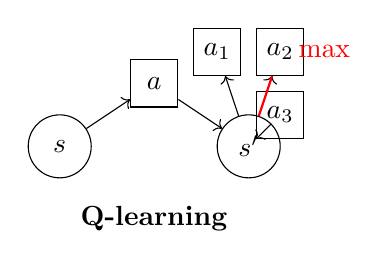
\begin{tikzpicture}[scale=0.8]
% Q-learning backup diagram
\node[draw, circle, minimum size=0.8cm] (s) at (0,0) {$s$};
\node[draw, circle, minimum size=0.8cm] (s_prime) at (3,0) {$s'$};
\node[draw, rectangle, minimum size=0.6cm] (a) at (1.5,1) {$a$};
\node[draw, rectangle, minimum size=0.6cm] (a1) at (2.5,1.5) {$a_1$};
\node[draw, rectangle, minimum size=0.6cm] (a2) at (3.5,1.5) {$a_2$};
\node[draw, rectangle, minimum size=0.6cm] (a3) at (3.5,0.5) {$a_3$};

\draw[->] (s) -- (a);
\draw[->] (a) -- (s_prime);
\draw[->] (s_prime) -- (a1);
\draw[->] (s_prime) -- (a2);
\draw[->] (s_prime) -- (a3);

% Highlight the max action
\draw[thick, red] (s_prime) -- (a2);
\node[red] at (4.2,1.5) {max};

\node[below] at (1.5,-0.8) {\textbf{Q-learning}};
\end{tikzpicture}
\hspace{1cm}
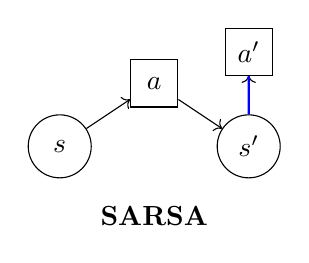
\begin{tikzpicture}[scale=0.8]
% SARSA backup diagram
\node[draw, circle, minimum size=0.8cm] (s) at (0,0) {$s$};
\node[draw, circle, minimum size=0.8cm] (s_prime) at (3,0) {$s'$};
\node[draw, rectangle, minimum size=0.6cm] (a) at (1.5,1) {$a$};
\node[draw, rectangle, minimum size=0.6cm] (a_prime) at (3,1.5) {$a'$};

\draw[->] (s) -- (a);
\draw[->] (a) -- (s_prime);
\draw[->] (s_prime) -- (a_prime);

% Highlight the selected action
\draw[thick, blue] (s_prime) -- (a_prime);

\node[below] at (1.5,-0.8) {\textbf{SARSA}};
\end{tikzpicture}
\end{center}

\begin{center}
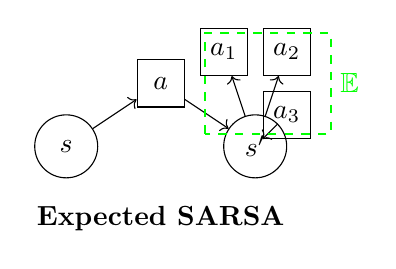
\begin{tikzpicture}[scale=0.8]
% Expected SARSA backup diagram
\node[draw, circle, minimum size=0.8cm] (s) at (0,0) {$s$};
\node[draw, circle, minimum size=0.8cm] (s_prime) at (3,0) {$s'$};
\node[draw, rectangle, minimum size=0.6cm] (a) at (1.5,1) {$a$};
\node[draw, rectangle, minimum size=0.6cm] (a1) at (2.5,1.5) {$a_1$};
\node[draw, rectangle, minimum size=0.6cm] (a2) at (3.5,1.5) {$a_2$};
\node[draw, rectangle, minimum size=0.6cm] (a3) at (3.5,0.5) {$a_3$};

\draw[->] (s) -- (a);
\draw[->] (a) -- (s_prime);
\draw[->] (s_prime) -- (a1);
\draw[->] (s_prime) -- (a2);
\draw[->] (s_prime) -- (a3);

% Show expectation over all actions
\draw[thick, green, dashed] (2.2,0.2) rectangle (4.2,1.8);
\node[green] at (4.5,1) {$\mathbb{E}$};

\node[below] at (1.5,-0.8) {\textbf{Expected SARSA}};
\end{tikzpicture}
\end{center}

\begin{itemize}
\item \textbf{Q-learning}: Uses $\max_a Q(s',a)$ (off-policy)
\item \textbf{SARSA}: Uses $Q(s',a')$ where $a'$ is chosen by policy (on-policy)
\item \textbf{Expected SARSA}: Uses $\sum_a \pi(a|s') Q(s',a)$ (expected value)
\end{itemize}

\subsection{Expected SARSA}
Expected Sarsa uses expected value under the current policy:

\begin{equation}
\begin{split}
Q&(S_t, A_t) \leftarrow Q(S_t, A_t) +  \\
 &\alpha [R_{t+1} + \gamma \sum_a \pi(a|S_{t+1}) Q(S_{t+1}, a) - Q(S_t, A_t)]
\end{split}
\end{equation}

\section{Function Approximation}
\section{n-step TD}
\begin{mdframed}
  
\textbf{n-step TD for estimating $V \approx v_\pi$}
\begin{algorithmic}
\State Input: policy $\pi$ to be evaluated
\State Algorithm parameters: step size $\alpha \in (0,1]$, positive integer $n$
\State Initialize $V(s)$ arbitrarily, for all $s \in \mathcal{S}$, except that $V(terminal) = 0$
\Repeat
  \State Initialize and store $S_0 \neq terminal$
  \State $T \leftarrow \infty$
  \For{$t = 0, 1, 2, \ldots$}
    \If{$t < T$}
      \State Take action according to $\pi(\cdot | S_t)$
      \State Observe and store the next reward as $R_{t+1}$ and the next state as $S_{t+1}$
      \If{$S_{t+1}$ is terminal}
        \State $T \leftarrow t + 1$
      \EndIf
    \EndIf
    \State $\tau \leftarrow t - n + 1$ (time whose estimate is being updated)
    \If{$\tau \geq 0$}
      \State $G \leftarrow \sum_{i=\tau+1}^{\min(\tau+n, T)} \gamma^{i-\tau-1} R_i$
      \If{$\tau + n < T$}
        \State $G \leftarrow G + \gamma^n V(S_{\tau+n})$ (bootstrap)
      \EndIf
      \State $V(S_\tau) \leftarrow V(S_\tau) + \alpha [G - V(S_\tau)]$
    \EndIf
  \EndFor
\Until{$\tau = T - 1$}
\end{algorithmic}
\end{mdframed}

So, when calculating, for example for a 3-step TD:
\begin{equation}
  V_{new}(S) \leftarrow V_{old}(S) + \alpha * ((R_{t} + \gamma * R_{t+1} + \gamma^2 * R_{t+2}) + \gamma^3 * V_{old}(T) - V_{old}(S))
\end{equation}
\section{General assignments}
\subsection{features + tiles}
You have 5 tilings of $10 * 10$ tiles. This means you have $10 * 10$ features in each tiling (one tile = one feature), and total $10 * 10 * 5 = 500$ features in all tilings.
\subsection{On tilings}
For each tiling, each state will be on exactly one tile from that tiling, there are no overlap tiles. 
So, for that tile, there is a one-hot "1" in the vector and the rest is 0. So, for 5 tilings, there are 5 1's in x(s).
\subsection{Picking a good step-size $\alpha$}
A rule of thumb for this is:
\begin{equation}
  a \doteq ( \tau \mathds{E} [ \textbf{x}^T \textbf{x}])^{-1}
\end{equation}
Supposing you want to learn about $\tau$ experiences with a substantially similar feature vector, with $\textbf{x}$ 
being a random feature vector chosen from the same distribution as input vectors will be in the Stochastic Gradient Descent.
\\
  
Say we have 5 tilings, for each feature vector $\textbf{x}$ there will be exactly 1 active tile in each tiling.
That means $\mathds{E}[\textbf{x}^t \textbf{x}] = 5$, regardless of distribution. so, with $\tau = 10$:
\begin{equation}
  \alpha = \frac{1}{10 \times 5} = 0.02
\end{equation}


\section{Policy Gradient}
\subsection{Stochastic Gradient Descent}
In SGD, we assume that states appeach in examples with the same distribution $\mu$, over which we are trying to minimize $\bar{VE}$.
A grood strategy is to minimize error, by adjusting weight vector after each sample in the direction that would reduce the most error:
\begin{equation}
  \textbf{w}_{t+1} = \textbf{w}_t - \frac{1}{2} \alpha \nabla [ v_{\pi}(S_t) - \hat{v}(S_t , \textbf{w}_t)]^2
\end{equation}
where $\alpha$ is step-size, $\nabla f(\textbf{w})$, is for any scalar expression $f(\textbf{w})$ that is a function of a vector.
It is the column vector of partial derivatives, with respect to the vector, or if you will, the gradient:
\begin{equation}
  \nabla f(\textbf{w}) \doteq (\frac{\partial f(\textbf{w})}{\partial w_1}, \frac{\partial f(\textbf{w})}{\partial w_2}, \cdots, \frac{\partial f(\textbf{w})}{\partial w_d})^T
\end{equation}
SGD methods are 'gradient methods' because the overall step in $\textbf{w}_t$ is proportional to the negative gradient of the example's squared error!
The general SGD method for state-value prediction:
\begin{equation}
\textbf{w}_{t+1} \doteq \textbf{w}_t + \alpha [U_t - \hat{v}(S_t, \textbf{w}_t)] \nabla \hat{v}(S_t, \textbf{w}_t)
\end{equation}

\textbf{Semi-gradient TD(0) for estimating $\hat{v} \approx v_{\pi}$}
\begin{algorithmic}
\State Input: the policy $\pi$ to be evaluated
\State Input: a differentiable function $\hat{v} : \mathcal{S}^+ \times \mathbb{R}^d \rightarrow \mathbb{R}$
\State Algorithm parameters: step size $\alpha > 0$
\State Initialize value-function weights $\mathbf{w} \in \mathbb{R}^d$ arbitrarily
\Repeat
  \State Initialize $S$ (start of episode)
  \Repeat
    \State $A \leftarrow$ action given by $\pi$ for $S$
    \State Take action $A$, observe $R$, $S'$
    \State $\mathbf{w} \leftarrow \mathbf{w} + \alpha [R + \gamma \hat{v}(S', \mathbf{w}) - \hat{v}(S, \mathbf{w})] \nabla \hat{v}(S, \mathbf{w})$
    \State $S \leftarrow S'$
  \Until{$S$ is terminal}
\Until{forever}
\end{algorithmic}

\end{multicols*}
\end{document}